% Copyright 2018, 2019, 2020, 2021 FIUS
%
% This file is part of theo-vorkurs-folien.
%
% theo-vorkurs-folien is free software: you can redistribute it and/or modify
% it under the terms of the GNU General Public License as published by
% the Free Software Foundation, either version 3 of the License, or
% (at your option) any later version.
%
% theo-vorkurs-folien is distributed in the hope that it will be useful,
% but WITHOUT ANY WARRANTY; without even the implied warranty of
% MERCHANTABILITY or FITNESS FOR A PARTICULAR PURPOSE.  See the
% GNU General Public License for more details.
%
% You should have received a copy of the GNU General Public License
% along with theo-vorkurs-folien.  If not, see <https://www.gnu.org/licenses/>.

% !TeX program = pdflatex
% !TeX spellcheck = de
% Copyright 2018-2022 FIUS
%
% This file is part of theo-vorkurs-folien.
%
% theo-vorkurs-folien is free software: you can redistribute it and/or modify
% it under the terms of the GNU General Public License as published by
% the Free Software Foundation, either version 3 of the License, or
% (at your option) any later version.
%
% theo-vorkurs-folien is distributed in the hope that it will be useful,
% but WITHOUT ANY WARRANTY; without even the implied warranty of
% MERCHANTABILITY or FITNESS FOR A PARTICULAR PURPOSE.  See the
% GNU General Public License for more details.
%
% You should have received a copy of the GNU General Public License
% along with theo-vorkurs-folien.  If not, see <https://www.gnu.org/licenses/>.

\documentclass[aspectratio=43,10pt]{beamer}

\usetheme[progressbar=frametitle]{metropolis}
\usepackage{appendixnumberbeamer}
\usepackage[ngerman]{babel}
\usepackage[utf8]{inputenc}
%\usepackage{t1enc}
\usepackage[T1]{fontenc}
\usepackage[sfdefault,scaled=.85,lf]{FiraSans}
\usepackage{newtxsf}

\usepackage{booktabs}
\usepackage[scale=2]{ccicons}
\usepackage{hyperref}

\usepackage{pgf}
\makeatletter
\@ifclasswith{beamer}{notes}{
  \usepackage{pgfpages}
  \setbeameroption{show notes on second screen}
}{}
\makeatother
\usepackage{tikz}
\usetikzlibrary{arrows,automata,positioning}
\usepackage{pgfplots}
\usepgfplotslibrary{dateplot}

\usepackage{xspace}
\newcommand{\themename}{\textbf{\textsc{metropolis}}\xspace}

\usepackage{blindtext}
\usepackage{graphicx}
\usepackage{subcaption}
\usepackage{comment}
\usepackage{mathtools}
\usepackage{amsmath}
\usepackage{centernot}
\usepackage{amssymb}
\usepackage{proof}
\usepackage{tabularx}
\renewcommand{\figurename}{Abb.}
\usepackage{marvosym}
\usepackage{mathtools}
\usepackage{qrcode}
\usepackage{advdate}

\newcommand\daynr{0}

\definecolor{ExColor}{HTML}{17819b}

\newcommand{\emptyWord}{\varepsilon}
\let \emptyset\varnothing
\newcommand{\SigmaStern}{\Sigma^{*}}
\newcommand{\absval}[1]{|#1|}
\newcommand{\defeq}{\vcentcolon=}
\newcommand{\eqdef}{=\vcentcolon}
\newcommand{\nimplies}{\centernot\implies}

\newcommand{\naturals}{\ensuremath{\mathbb{N}}}
\newcommand{\integers}{\ensuremath{\mathbb{Z}}}
\newcommand{\rationals}{\ensuremath{\mathbb{Q}}}
\newcommand{\reals}{\ensuremath{\mathbb{R}}}
\newcommand{\iffspace}{\ensuremath{\iff\;}}

\setbeamertemplate{footline}[text line]
{\parbox{\linewidth}{Fachgruppe Informatik\hfill\insertpagenumber\hfill Vorkurs Theoretische Informatik\vspace{0.2in}}}

\newcommand{\Center}[1]{
  \begin{frame}<handout:0>[standout]
    #1
  \end{frame}
}

% Fix section pages in appendix
\AtBeginDocument{%
  \apptocmd{\appendix}{%
    \setbeamertemplate{section page}[simple]%
  }{}{}
}

\addtobeamertemplate{block begin}{}{\vskip 0em}
\addtobeamertemplate{block alerted begin}{}{\vskip 0em}
\addtobeamertemplate{block example begin}{}{\vskip 0em}

% Copyright 2018-2022 FIUS
%
% This file is part of theo-vorkurs-folien.
%
% theo-vorkurs-folien is free software: you can redistribute it and/or modify
% it under the terms of the GNU General Public License as published by
% the Free Software Foundation, either version 3 of the License, or
% (at your option) any later version.
%
% theo-vorkurs-folien is distributed in the hope that it will be useful,
% but WITHOUT ANY WARRANTY; without even the implied warranty of
% MERCHANTABILITY or FITNESS FOR A PARTICULAR PURPOSE.  See the
% GNU General Public License for more details.
%
% You should have received a copy of the GNU General Public License
% along with theo-vorkurs-folien.  If not, see <https://www.gnu.org/licenses/>.



% Configuration for slides

% The date of the first day of the Theo-Vorkurs in Format dd/mm/yyyy
\SetDate[10/10/2022]

% Invite URL to the Ersti-Telegram-Group. Used for text on slide as well as QR-Code
\newcommand\telegramurl{https://t.me/+Q92w5biyY903NjEy}

% The url to the handout of the current day with the current day as argument. Used for the qr-code in the slides. 
\newcommand{\handouturl}[1]{https://fius.de/wp-content/uploads/2022/10/day-#1-handout.pdf}


\title{Vorkurs Theoretische Informatik}
\subtitle{Einführung in reguläre Sprachen}
\date{Donnerstag, 14.10.2021}
\author{Arbeitskreis Theo Vorkurs}
\institute{Fachgruppe Informatik}
% \titlegraphic{\hfill\includegraphics[height=1.5cm]{logo.pdf}}

\begin{document}

\maketitle

\begin{frame}[fragile]{Übersicht}
  \setbeamertemplate{section in toc}[sections numbered]
  \tableofcontents%[hideallsubsections]
\end{frame}

\section{Chomsky-Hierarchie}

\begin{frame}[fragile]{Manche Sprachen sind schwerer zu beschreiben als andere}
    Wenn wir unsere Grammatiken einschränken, können wir nicht mehr alle Sprachen beschreiben.
    \metroset{block=fill}
    \begin{exampleblock}{Beispiel}
        Mit der Einschränkung\\
        \emph{Alle Produktionsregeln müssen der Form \alert{A $\to$ a oder A $\to$ aB} entsprechen, wobei A, B $\in$ V und a $\in \Sigma$}.\\
        können wir Sprachen wie $L_1 = \{a^n \mid n \in \naturals\}$ beschreiben,\\ aber nicht mehr Sprachen wie $L_1 = \{a^nb^n \mid n \in \naturals\}$.\\
        \alert{Achtung:} ist $\emptyWord \in L$, ist auch $S\to\emptyWord$ erlaubt, sofern $S$ nicht auf der rechten Seite einer Produktion vorkommt.
    \end{exampleblock}
    $\leadsto$ Sprachen, die wir mit dieser starken Einschränkung beschreiben können, nennen wir \alert{\emph{regulär}} oder vom \alert{\emph{Typ 3}}.\\
    Es gibt weitere Typen $\leadsto$ Mehr dazu in der Vorlesung
\end{frame}

\begin{frame}[fragile]{Manche Sprachen sind schwerer zu beschreiben als andere}
    \begin{center}
        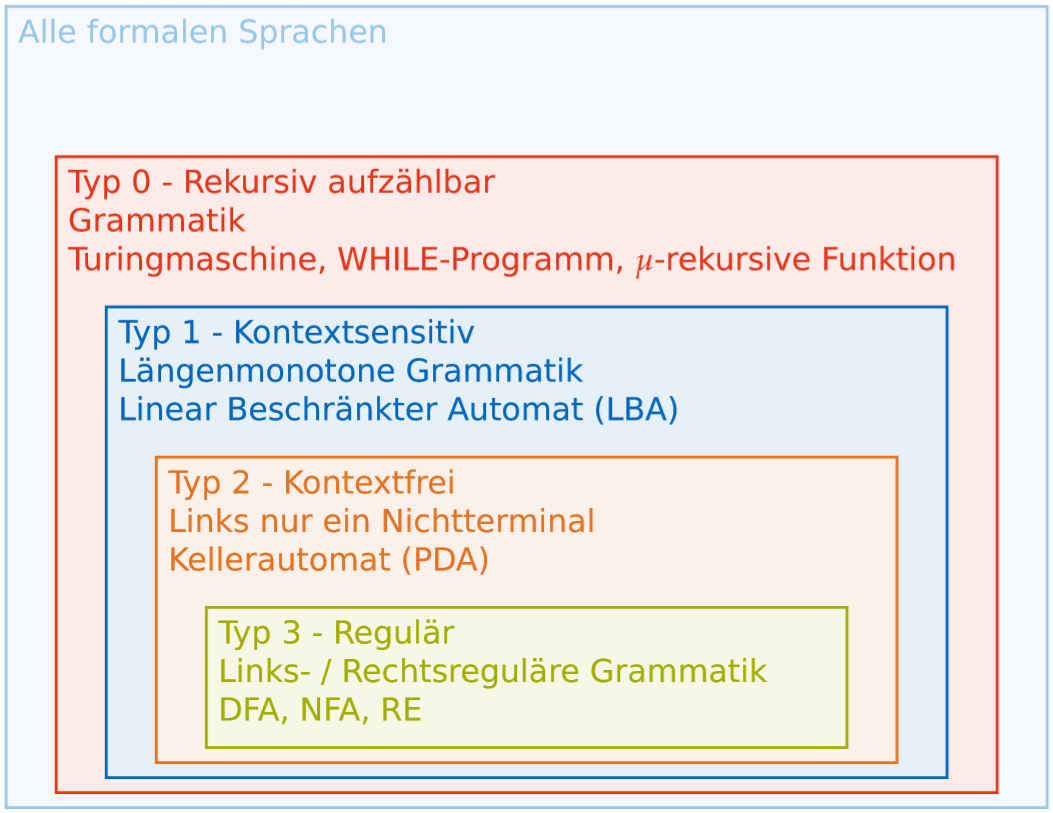
\includegraphics[width=0.75\textwidth]{../figures/Chomsky.png}
    \end{center}
\end{frame}

{\setbeamercolor{palette primary}{bg=ExColor}
\begin{frame}{Reguläre Grammatik}
    \begin{alertblock}{Aufgaben}
    Finde eine reguläre Grammatik für die folgenden Sprachen
    \end{alertblock}
    \metroset{block=fill}
    \begin{block}{Normal}
    \begin{itemize}
        \item $L_1 = \{a^{2n} \mid n\in\naturals\}$
        \item $L_2 = \{a^nb^m \mid n, m\in\naturals\}$
        \item $L_3 = \{uv \mid u\in\{a,b\}^\ast,\ v\in\{c,d\}\}$
        \item $L_4 = \{w \mid |w| = 3, w\in \{a,b,c\}^*\}$
    \end{itemize}
    \end{block}
    \begin{block}{Etwas Schwerer}
    \begin{itemize}
        \item $L_5 = \{a^n \mid n \equiv 1 \mod 3\}$
        \item $L_6 = \{uv\mid u\in\{\text{\Rewind, \MoveUp, \Forward, \MoveDown}\}^\ast,\;v\in\{\text{\Stopsign}\}\}$
        \item $L_7 = \{w \in \{a,b,c\}^* \mid |w|_a = 3, |w|_b = 1\}$
    \end{itemize}
    \end{block}
\end{frame}
}

{\setbeamercolor{palette primary}{bg=ExColor}
\begin{frame}{Lösung}
    \begin{itemize}
        \item<1-> \alert<1>{$P_1 = \{S \to aA \mid \emptyWord,\ A \to aB \mid a,\ B \to aA\}$}
        \item<2-> \alert<2>{$P_2 = \{S \to aA \mid bB \mid b \mid a \mid \emptyWord,\ A \to aA \mid bB \mid b \mid a ,\ B \to bB \mid b\}$}
        \item<3-> \alert<3>{$P_3 = \{S \to aS \mid bS \mid c \mid d\}$}
        \item<4-> \alert<4>{$P_4 = \{S \to aA \mid bA \mid cA,\ A \to aB \mid bB \mid cB,\ B \to a \mid b \mid c\}$}
        \item<5-> \alert<5>{$P_5 = \{S \to aA \mid a,\ A \to aB,\ B \to aS\}$}
        \item<6-> \alert<6>{$P_6 = \{S \to \text{\Rewind}S \mid \text{\MoveUp}S \mid \text{\Forward}S \mid \text{\MoveDown}S \mid \text{\Stopsign}\}$}
    \end{itemize}
\end{frame}
}

{\setbeamercolor{palette primary}{bg=ExColor}
\begin{frame}{Lösung}
        \begin{itemize}
            \item 
                \alert<1>{
                $P_7 = \{S \to cS \mid aA_1 \mid bB_0,$\\
                \vspace*{0.9mm}
                \hspace*{7mm}
                $\begin{aligned}
                A_1 &\to cA_1 \mid aA_2 \mid bB_1,\\
                A_2 &\to cA_2 \mid aA_3 \mid bB_2,\\
                A_3 &\to cA_3 \mid bB_3 \mid b,\\
                B_0 &\to cB_0 \mid aB_1,\\
                B_1 &\to cB_1 \mid aB_2,\\
                B_2 &\to cB_2 \mid aB_3 \mid a,\\
                B_3 &\to cB_3 \mid cC \mid c,\\
                C_{\;} &\to cC_{\;}\mid c\}
                \end{aligned}
                $}
        \end{itemize}
\end{frame}
}


\Center{Murmelpause}

\section{Automaten}

\begin{frame}[fragile]{Reguläre Sprachen anders beschreiben}
    Wir können reguläre Sprachen auch graphisch beschreiben.\\
    Dafür nutzen wir \alert{endliche Automaten}.\\
    Ein Automat prüft Wörter und entscheidet, ob sie Teil der Sprache sind oder nicht.\\
    $\leadsto$ Wir nennen das \alert{\emph{akzeptieren}}, bzw. nicht akzeptieren.
    \begin{alertblock}{Funktionsweise}
        \begin{enumerate}
            \item Ein Wort wird in den Automat eingegeben
            \item Wort wird zeichenweise abgearbeitet
            \item Nach jedem Zeichen wird der Automat in einen Zustand überführt, der bestimmt, wie fortgefahren wird
            \item Befindet sich der Automat in einem \emph{Endzustand}, sobald das Wort abgearbeitet wurde, akzeptiert der Automat das Wort.
        \end{enumerate}
    \end{alertblock}
\end{frame}

\subsection{NEA}
\begin{frame}[fragile]{Bestandteile eines endlichen Automaten}
    Der Automat kann als gerichteter Graph notiert werden.\\
    Wir konstruieren ihn aus den folgenden Komponenten:
    \only<1|handout:1>{
        \begin{alertblock}{Startzustand}
            Im Startzustand wird das Wort eingegeben.\\
            \begin{center}
                \begin{tikzpicture}[->,>=stealth',shorten >=1pt,auto,node distance=2cm,semithick]
                    \node[initial,state](q0){$q_0$};
                \end{tikzpicture}
            \end{center}
        \end{alertblock}
    }
    \only<2|handout:1>{
        \begin{alertblock}{Zustandsübergang}
            Wird das Zeichen auf dem Übergang \emph{gelesen}, geht der Automat in den folgenden Zustand über.\\
            \begin{center}
                \begin{tikzpicture}[->,>=stealth',shorten >=1pt,auto,node distance=2cm,semithick]
                    \node[state](qi){$q_i$};
                    \node[state](qj)[right of=qi]{$q_j$};
                    \path (qi) edge node {$a$} (qj);
                \end{tikzpicture}
            \end{center}
        \end{alertblock}
    }
    \only<3|handout:2>{
        \begin{alertblock}{Endzustand}
            Falls sich der Automat in diesem Zustand befindet, und das Wort abgearbeitet ist, wird das Wort akzeptiert.\\
            \begin{center}
                \begin{tikzpicture}[->,>=stealth',shorten >=1pt,auto,node distance=2cm,semithick]
                    \node[accepting,state](qe){$q_E$};
                \end{tikzpicture}
            \end{center}
            \emph{Anmerkung: }Unter Umständen sind mehrere hiervon nötig
        \end{alertblock}
    }
\end{frame}

\begin{frame}[fragile]{Beispiel}
    \begin{exampleblock}{$L=\{axb \mid x\in\{a,b\}^\ast\}$}
        \vspace{0.3cm}
        \begin{tikzpicture}[->,>=stealth',shorten >=1pt,auto,node distance=2cm,
                semithick]
            %\tikzstyle{every state}=[fill=ExColor,draw=none,text=white]

            \node<1,3-> [initial,state]         (1)               {$q_0$};
            \node<2>    [initial,state,orange]  (1)               {$q_0$};
            \node       [state]                 (2) [right of=1]  {$q_1$};
            \node<1-8>  [state,accepting]       (3) [right of=2]  {$q_E$};
            \node<9>    [state,accepting,orange](3) [right of=2]  {$q_E$};

            \path<1,2,9>
            (1) edge                node {a}  (2)
            (2) edge [loop above]   node {a,b}(2)
            edge                node {b}  (3);
            \path<3>
            (1) edge [orange]       node {a}  (2)
            (2) edge [loop above]   node {a,b}(2)
            edge                node {b}  (3);
            \path<4,5,6,7>
            (1) edge                     node {a}  (2)
            (2) edge [loop above,orange] node {a,b}(2)
            edge                     node {b}  (3);
            \path<8>
            (1) edge                node {a}  (2)
            (2) edge [loop above]   node {a,b}(2)
            edge [orange]       node {b}  (3);
        \end{tikzpicture}
    \end{exampleblock}
    \onslide<2->{
        \begin{exampleblock}{Worteingabe:} \alert<3>{a}\alert<4>{a}\alert<5>{b}\alert<6>{a}\alert<7>{b}\alert<8>{b} $\in L$\only<1-8>{?} \only<9>{$\leadsto$ \alert{akzeptiert}
            }
        \end{exampleblock}}
\end{frame}

\begin{frame}{Beispiel: Automat}
    Gegeben ist eine Sprache L. Gesucht ist ein Automat M, der \textbf{genau} die Wörter aus L akzeptiert.
    \vspace{0.5cm}
    % \only<1>{
    % \begin{alertblock}{$L_1 = \{a^{2n} \mid n\in\naturals\}$}
    % \begin{tikzpicture}[->,>=stealth',shorten >=1pt,auto,node distance=2cm,semithick]
    %         \node   [initial,state,accepting]                   (1) {$q_0$};
    %         \node   [state]                     [right of=1]    (2) {$q_1$};
    %         \node   [state, accepting]          [right of=2]    (3) {$q_2$};

    %         \path
    %                 (1) edge node {a} (2);

    %         \path
    %                 (2) edge [bend left] node {a} (3);

    %         \path
    %                 (3) edge [bend left] node {a} (2);
    %     \end{tikzpicture}
    % \end{alertblock}
    % }
    \only<1>{
        \begin{alertblock}{$L_1 = \{uv \mid u\in\{a,b\}^\ast,\;v\in\{c,d\}\}$}
            \begin{tikzpicture}[->,>=stealth',shorten >=1pt,auto,node distance=2cm,semithick]
                \node   [initial,state]                             (1) {$q_0$};
                \node   [state,accepting]           [right of=1]    (2) {$q_1$};

                \path   (1) edge node {c,d} (2)
                (1) edge [loop above] node {a,b} (1);
            \end{tikzpicture}
        \end{alertblock}
    }

\end{frame}

{\setbeamercolor{palette primary}{bg=ExColor}
\begin{frame}{Denkpause}
    \begin{small}
        \begin{alertblock}{knifflige Aufgabe}
            Wir entwerfen einen Automat zur Aufzugskontrolle.
            Der Aufzug hat folgende Möglichkeiten:\\
            $\Sigma =\{$\begin{footnotesize}
                \framebox{EG$\nearrow$1.OG} , \framebox{EG$\nearrow$2.OG} , \framebox{1.OG$\searrow$EG} , \framebox{1.OG$\nearrow$2.OG} , \framebox{2.OG$\searrow$EG} , \\\qquad\quad\;\framebox{2.OG$\searrow$1.OG} , \framebox{OFF}
            \end{footnotesize}$\}$
            \begin{itemize}
                \item Der Aufzug startet vom Erdgeschoss und darf sich nur aus Stockwerken bewegen, in denen er sich befindet.
                \item Der Aufzug kann nur im Erdgeschoss ausgeschaltet werden. Er kann dann keine Bewegung durchführen.
                \item Der Aufzug muss ausgeschaltet werden.
            \end{itemize}
        \end{alertblock}
        % \begin{footnotesize}
        %     \framebox{EG$\nearrow$2.OG} \framebox{2.OG$\searrow$EG} \framebox{OFF} $\in L$\\
        %     \framebox{2.OG$\searrow$EG} \framebox{OFF} \framebox{EG$\nearrow$1.OG} $\notin L$\\
        % \end{footnotesize}
        \alert{Zeichne einen Automaten an, dessen akzeptierte Sprache genau die Menge der korrekten Abläufe ist.}
    \end{small}
\end{frame}

\begin{frame}<handout:0>{Lösung}
    \begin{center}
        \begin{tikzpicture}[->,>=stealth',shorten >=1pt,auto,node distance=3.2cm,semithick]
            \node [initial,state]   (0)              {$q_0$};
            \node [state]           (1) [above of=0] {$q_1$};
            \node [state]           (2) [above of=1] {$q_2$};
            \node [state,accepting] (E) [right of=0] {$q_E$};

            \path   (0) edge [bend left=10] node [rotate=90,above] {\footnotesize\framebox{EG$\nearrow$1.OG}} (1)
            edge [below]      node {\footnotesize\framebox{OFF}} (E)
            edge [bend left=70] node {\footnotesize\framebox{EG$\nearrow$2.OG}} (2)
            (1) edge [bend left=10] node [rotate=90,above] {\footnotesize\framebox{1.OG$\nearrow$2.OG}} (2)
            edge [bend left=10] node [rotate=90,below] {\footnotesize\framebox{1.OG$\searrow$EG}} (0)
            (2) edge [bend left=10] node [rotate=90,below] {\footnotesize\framebox{2.OG$\searrow$1.OG}}(1)
            edge [bend left=70] node {\footnotesize\framebox{2.OG$\searrow$EG}} (0);
        \end{tikzpicture}
    \end{center}
\end{frame}
}

{\setbeamercolor{palette primary}{bg=ExColor}
\begin{frame}{Denkpause}
    \begin{alertblock}{Aufgaben}
        Finde Automaten, die \textbf{genau} folgende Sprachen erkennen.
    \end{alertblock}
    \metroset{block=fill}
    \begin{block}{Normal}
        \begin{itemize}
            \item $L_1 = \{a^nb^m \mid n, m\in\naturals\}$
            \item $L_2 = \{w \mid |w| = 3, w\in \{a,b,c\}^*\}$
            \item $L_3 = \{uv \mid u\in\{\text{\Rewind, \MoveUp, \Forward, \MoveDown}\}^\ast,\;v\in\{\text{\Stopsign}\}\}$
        \end{itemize}
    \end{block}
    \begin{block}{Etwas Schwerer}
        \begin{itemize}
            \item $L_4 = \{a^n \mid n \equiv 1 \bmod 3\}$
            \item $L_5 = \{w \in \{a,b,c\}^* \mid |w|_a = 3, |w|_b = 1\}$
            \item $L_6=\{w \in \{a,b\}^* \mid |w|_a \equiv |w|_b \bmod 3\}$
        \end{itemize}
    \end{block}
\end{frame}
}



{\setbeamercolor{palette primary}{bg=ExColor}
\begin{frame}<handout:0>{Lösung}
    % \begin{itemize}[<+- | alert@+>]
    %     \item 
    \onslide<1->{\alert<1>{
        % \item
        \begin{tikzpicture}[->,>=stealth',shorten >=1pt,auto,node distance=2cm,semithick]
            \node   [initial,state,accepting]                   (1) {$q_0$};
            \node   [state,accepting]           [right of=1]    (2) {$q_1$};

            \path   (1) edge node {b} (2)
            (1) edge [loop above] node {a} (1);

            \path   (2) edge [loop above] node {b} (2);
        \end{tikzpicture}
    }}
    \vspace{0.2cm}
    \onslide<2->{\alert<2>{
        \begin{tikzpicture}[->,>=stealth',shorten >=1pt,auto,node distance=2cm,semithick]
            \node   [initial,state]                             (1) {$q_0$};
            \node   [state]             [right of=1]            (2) {$q_1$};
            \node   [state]             [right of=2]            (3) {$q_2$};
            \node   [state,accepting]   [right of=3]            (4) {$q_3$};

            \path   (1) edge node {a,b,c} (2);
            \path   (2) edge node {a,b,c} (3);
            \path   (3) edge node {a,b,c} (4);
        \end{tikzpicture}
    }}
    \vspace{0.2cm}
    \onslide<3->{\alert<3>{
        \begin{tikzpicture}[->,>=stealth',shorten >=1pt,auto,node distance=2cm,semithick]
            \node   [initial,state]         (1) {$q_0$};
            \node   [state,accepting]   [right of=1]       (2) {$q_1$};

            \path   (1) edge    [loop above]    node    {\text{\Rewind, \MoveUp, \Forward, \MoveDown}} (1)
            (1) edge                    node    {$\text{\Stopsign}$}   (2);
        \end{tikzpicture}}}
    \vspace{0.2cm}
    \onslide<4->{\alert<4>{
        \begin{tikzpicture}[->,>=stealth',shorten >=1pt,auto,node distance=2cm,semithick]
            \node   [initial,state]                             (1) {$q_0$};
            \node   [state,accepting]   [right of=1]            (2) {$q_1$};
            \node   [state]             [right of=2]            (3) {$q_2$};

            \path   (1) edge node {a} (2);
            \path   (2) edge node {a} (3);
            \path   (3) edge [bend left] node {a} (1);
        \end{tikzpicture}
    }}
    % \end{itemize}
\end{frame}
}

{\setbeamercolor{palette primary}{bg=ExColor}
\begin{frame}<handout:0>{Lösung}
    \onslide<1->{\alert<1>{
        \begin{tikzpicture}[->,>=stealth',shorten >=1pt,auto,node distance=1.5cm,semithick]
            \node   [initial,state]                             (1) {$q_0$};
            \node   [state]             [right of=1]            (2) {$q_1$};
            \node   [state]             [right of=2]            (3) {$q_2$};
            \node   [state]             [right of=3]            (4) {$q_3$};
            \node   [state]             [below of=1]             (5) {$q_4$};
            \node   [state]             [below of=2]             (6) {$q_5$};
            \node   [state]             [below of=3]             (7) {$q_6$};
            \node   [state, accepting]  [below of=4]             (8) {$q_7$};

            \path   (1) edge node {a} (2)
            (1) edge node {b} (5)
            (1) edge [loop above] node {c} (1);

            \path   (2) edge node {a} (3)
            (2) edge node {b} (6)
            (2) edge [loop above] node {c} (2);

            \path   (3) edge node {a} (4)
            (3) edge node {b} (7)
            (3) edge [loop above] node {c} (3);

            \path   (4) edge node {b} (8)
            (4) edge [loop above] node {c} (4);

            \path   (5) edge node {a} (6)
            (5) edge [loop below] node {c} (5);

            \path   (6) edge node {a} (7)
            (6) edge [loop below] node {c} (6);

            \path   (7) edge node {a} (8)
            (7) edge [loop below] node {c} (7);

            \path   (8) edge [loop below] node {c} (8);
        \end{tikzpicture}
    }}
\end{frame}
}

{\setbeamercolor{palette primary}{bg=ExColor}
\begin{frame}<handout:0>{Lösung}
    \onslide<1->{\alert<1>{
        \begin{tikzpicture}[->,>=stealth',shorten >=1pt,auto,node distance=4cm,semithick]
            \node   [initial,state,accepting]                             (1) {$q_0$};
            \node   [state]             [right of=1]            (2) {$q_1$};
            \node   [state]             [below of=1]            (3) {$q_2$};

            \path   (1) edge [bend right] node {a} (2)
            (1) edge [bend right] node {b} (3);
            \path   (2) edge node {a} (3)
            (2) edge [bend right] node {b} (1);
            \path   (3) edge [bend right] node {a} (1)
            (3) edge [bend right=60] node {b} (2);
        \end{tikzpicture}
    }}
\end{frame}
}


\Center{Murmelpause}

% Copyright 2018-2022 FIUS
%
% This file is part of theo-vorkurs-folien.
%
% theo-vorkurs-folien is free software: you can redistribute it and/or modify
% it under the terms of the GNU General Public License as published by
% the Free Software Foundation, either version 3 of the License, or
% (at your option) any later version.
%
% theo-vorkurs-folien is distributed in the hope that it will be useful,
% but WITHOUT ANY WARRANTY; without even the implied warranty of
% MERCHANTABILITY or FITNESS FOR A PARTICULAR PURPOSE.  See the
% GNU General Public License for more details.
%
% You should have received a copy of the GNU General Public License
% along with theo-vorkurs-folien.  If not, see <https://www.gnu.org/licenses/>.

\begin{frame}[fragile]{Verschiedene endliche Automaten}
    \begin{alertblock}{NEA}
        Beim Lesen eines Wortes ist es manchmal unklar, welchen Übergang der Automat nehmen soll.\\
        $\leadsto$ Der Automat ist \emph{\alert{nichtdeterministisch}}.
    \end{alertblock}
    \begin{alertblock}{DEA}
        Wir können unsere Möglichkeiten so einschränken, dass bei jedem Zeichen eindeutig ist, welcher Übergang genutzt wird.\\
        $\leadsto$ Der Automat ist \alert{\emph{deterministisch}}.
    \end{alertblock}
\end{frame}

\begin{frame}[fragile]{Unterschied NEA und DEA}
    Bildlich kann man den Unterschied zwischen NEA und DEA an verschiedenen Merkmalen erkennen:
    \begin{alertblock}{Mehrere Möglichkeiten bei Übergängen:}
        \begin{center}
            \begin{tikzpicture}[->, >=stealth, shorten >=1pt, semithick]
                \node[state]         (1)                            {$q_i$};
                \node[state]         (2) [above right=0.7cm and 2cm of 1]   {$q_j$};
                \node[state]         (3) [below right=0.7cm and 2cm of 1]   {$q_k$};

                \path
                (1) edge                node[above] {$a$}  (2)
                edge                node[below] {$a,b$}(3);
            \end{tikzpicture}
        \end{center}
        Bei einem DEA wäre nur ein Weg mit einem \alert{$a$} von dem Zustand $q_i$ aus erlaubt!
    \end{alertblock}
\end{frame}

\begin{frame}[fragile]{Unterschied NEA und DEA}
    Bildlich kann man den Unterschied zwischen NEA und DEA an verschiedenen Merkmalen erkennen:
    \begin{alertblock}{Nicht definierte Übergänge}
        \begin{center}
            \begin{tikzpicture}[->, >=stealth, shorten >=1pt, semithick]
                \node[state]         (1)                {$q_i$};
                \node[state]         (2) [right = 2cm of 1]   {$q_j$};

                \path
                (1) edge[bend left]  node[above] {$a$}  (2)
                (2) edge[bend left]  node[below] {$a,b$}(1);
            \end{tikzpicture}
        \end{center}
        Bei einem DEA müsste ein Übergang mit \alert{$b$} für den Zustand $q_i$ definiert werden!
    \end{alertblock}
\end{frame}

\begin{frame}[fragile]{Unterschied NEA und DEA}
    Bildlich kann man den Unterschied zwischen NEA und DEA an verschiedenen Merkmalen erkennen:
    \begin{alertblock}{Mehrere Startzustände}
        \begin{center}
            \begin{tikzpicture}[->, >=stealth, shorten >=1pt, semithick]
                \node[state, initial]         (1)                      {$q_0$};
                \node[state, initial]         (2) [below = 1.5cm of 1]   {$\tilde{q}_0$};
                \node[state]                  (3) [below right= 0.75cm and 2cm of 1]   {$q_1$};

                \path
                (1) edge node[above] {$a$}  (3)
                edge[loop above] node[above] {$b$} (1)
                (2) edge node[below] {$a,b$}(3);
            \end{tikzpicture}
        \end{center}
        Ein DEA muss \alert{genau einen} Startzustand besitzen!
    \end{alertblock}
\end{frame}

\begin{frame}{Wann wird ein Wort akzeptiert?}
    Ein Wort $w \in \Sigma^*$ wird von einem NEA akzeptiert, wenn es \alert{mindestens einen} akzeptierenden Pfad gibt.
    \begin{alertblock}{Beispiel}
        Welche Zustände können erreicht werden, wenn $w = aaba$ eingelesen wird?\\
        \begin{tikzpicture}[->, >=stealth, shorten >=1pt, semithick]
        	%normal
            \node<1,11,14,16,18,19->	[state, initial]   (0)                    {$q_0$};
            \node<1-10,12-13,15,17,19->	[state, accepting] (1) [right = 2cm of 0] {$q_1$};
            \node<1-18>	[state]            (2) [right = 2cm of 1] {$q_2$};
            %alerted
            \node<2-10,12-13,15,17|handout:0> [state, initial,orange]   (0)                    {$q_0$};
            \node<11,14,16,18|handout:0>	[state, accepting,orange] (1) [right = 2cm of 0] {$q_1$};
            \node<19-|handout:0>		[state,orange]            (2) [right = 2cm of 1] {$q_2$};
            
            %normal
			\path<1,11,16>
			(0) edge[loop above]    node[above] {$a,b$}   (0)
			(0) edge[bend right]    node[below] {$a$}     (1)
			(1) edge[bend right]    node[above] {$b$}     (0)
			(1) edge                node[above] {$a$}     (2)
			(2) edge[loop above]    node[above] {$a,b$}   (2);
			%alerted
            \path<2-9,12|handout:0>
            (0) edge[loop above,orange] node[above] {$a,b$}   (0)
            (0) edge[bend right]   		node[below] {$a$}     (1)
            (1) edge[bend right]    	node[above] {$b$}     (0)
            (1) edge                	node[above] {$a$}     (2)
            (2) edge[loop above]    	node[above] {$a,b$}   (2);
            \path<10,13,15,17|handout:0>
            (0) edge[loop above]    	node[above] {$a,b$}   (0)
            (0) edge[bend right,orange] node[below] {$a$}     (1)
            (1) edge[bend right]    	node[above] {$b$}     (0)
            (1) edge                	node[above] {$a$}     (2)
            (2) edge[loop above]    	node[above] {$a,b$}   (2);
            \path<14|handout:0>
            (0) edge[loop above]    	node[above] {$a,b$}   (0)
            (0) edge[bend right] 		node[below] {$a$}     (1)
            (1) edge[bend right,orange] node[above] {$b$}     (0)
            (1) edge                	node[above] {$a$}     (2)
            (2) edge[loop above]    	node[above] {$a,b$}   (2);
            \path<18|handout:0>      
            (0) edge[loop above] node[above] {$a,b$}   (0)
            (0) edge[bend right] node[below] {$a$}     (1)
            (1) edge[bend right] node[above] {$b$}     (0)
            (1) edge[orange]     node[above] {$a$}     (2)
            (2) edge[loop above] node[above] {$a,b$}   (2);
            \path<19-|handout:0>
            (0) edge[loop above]    	node[above] {$a,b$}   (0)
            (0) edge[bend right] 		node[below] {$a$}     (1)
            (1) edge[bend right] 		node[above] {$b$}     (0)
            (1) edge                	node[above] {$a$}     (2)
            (2) edge[loop above,orange] node[above] {$a,b$}   (2);
        \end{tikzpicture}
        \vspace*{-5mm}
        \begin{center}
            \begin{enumerate}
                \item[i)]<2-> 
                	\alert<2|handout:0>{$q_0 \rightarrow$}
                	\alert<3|handout:0>{$q_0 \rightarrow$} 
                	\alert<4|handout:0>{$q_0 \rightarrow$} 
                	\alert<5|handout:0>{$q_0 \rightarrow$} 
                	\alert<6|handout:0>{$q_0$} 
                \item[ii)]<7-> 
                	\alert<7|handout:0>{$q_0 \rightarrow$} 
	                \alert<8|handout:0>{$q_0 \rightarrow$} 
	                \alert<9|handout:0>{$q_0 \rightarrow$} 
	                \alert<10|handout:0>{$q_0 \rightarrow$} 
	                \alert<11|handout:0>{$q_1$} (Endzustand erreicht)
                \item[iii)]<12-> 
                	\alert<12|handout:0>{$q_0 \rightarrow$} 
	                \alert<13|handout:0>{$q_0 \rightarrow$} 
	                \alert<14|handout:0>{$q_1 \rightarrow$} 
	                \alert<15|handout:0>{$q_0 \rightarrow$} 
	              	\alert<16|handout:0>{$q_1$} (Endzustand erreicht)
                \item[iv)]<17-> 
                	\alert<17|handout:0>{$q_0 \rightarrow$} 
	                \alert<18|handout:0>{$q_1 \rightarrow$} 
	                \alert<19|handout:0>{$q_2 \rightarrow$} 
	                \alert<20|handout:0>{$q_2 \rightarrow$} 
	                \alert<21|handout:0>{$q_2$} 
            \end{enumerate}
        \end{center}
    \end{alertblock}
\end{frame}

% Copyright 2018, 2019, 2020, 2021 FIUS
%
% This file is part of theo-vorkurs-folien.
%
% theo-vorkurs-folien is free software: you can redistribute it and/or modify
% it under the terms of the GNU General Public License as published by
% the Free Software Foundation, either version 3 of the License, or
% (at your option) any later version.
%
% theo-vorkurs-folien is distributed in the hope that it will be useful,
% but WITHOUT ANY WARRANTY; without even the implied warranty of
% MERCHANTABILITY or FITNESS FOR A PARTICULAR PURPOSE.  See the
% GNU General Public License for more details.
%
% You should have received a copy of the GNU General Public License
% along with theo-vorkurs-folien.  If not, see <https://www.gnu.org/licenses/>.

\subsection{DEA}
\begin{frame}[fragile]{Deterministische endliche Automaten}
    \begin{alertblock}{Wir beschränken unseren Automaten folgendermaßen:}
        Von \alert{jedem Zustand} muss \alert{genau ein} Übergang für \alert{jedes $a\in\Sigma$} ausgehen.
    \end{alertblock}
    %\vspace{0.3}
    \onslide<2->{
        Um dies zu ermöglichen führen wir eine neue Komponente ein:
        \begin{alertblock}{Fangzustand}
            Dieser Zustand kann nicht verlassen werden.\\
            Falls der Automat in diesem Zustand landet, kommt er nicht mehr raus. Das Wort kann nicht akzeptiert werden.
            \begin{center}
                \begin{tikzpicture}[->,>=stealth',shorten >=1pt,auto,node distance=2cm,semithick]
                    \node[state](qi){$q_f$};
                    \path (qi) edge [loop right] node {$x \in \Sigma$} (B);
                \end{tikzpicture}
            \end{center}
        \end{alertblock}
    }
\end{frame}

\begin{frame}[fragile]{Beispiel}
    \begin{exampleblock}{$L=\{axb \mid x\in\{a,b\}^\ast\}$}
        \vspace{0.3cm}
        \begin{tikzpicture}[->,>=stealth,shorten >=1pt,auto,node distance=2cm,
                semithick]
            %\tikzstyle{every state}=[fill=ExColor,draw=none,text=white]

            \node<1,3-> [initial,state]         (1)               {$q_0$};
            \node<2>    [initial,state,orange]  (1)               {$q_0$};
            \node       [state]                 (2) [right of=1]  {$q_1$};
            \node<1-8>  [state,accepting]       (3) [right of=2]  {$q_E$};
            \node<9>    [state,accepting,orange](3) [right of=2]  {$q_E$};
            \node       [state]                 (4) [below of=1]  {$q_f$};

            \path<1,2,9>
            (1) edge                node {$a$}  (2)
            edge                node {$b$}  (4)
            (2) edge [loop above]   node {$a$}  (2)
            edge [bend left]    node {$b$}  (3)
            (4) edge [loop right]   node {$a,b$}(4)
            (3) edge [loop above]   node {$b$}  (3)
            edge [bend left]    node {$a$}  (2);
            \path<3>
            (1) edge [orange]       node {$a$}  (2)
            edge                node {$b$}  (4)
            (2) edge [loop above]   node {$a$}  (2)
            edge [bend left]    node {$b$}  (3)
            (4) edge [loop right]   node {$a,b$}(4)
            (3) edge [loop above]   node {$b$}  (3)
            edge [bend left]    node {$a$}  (2);
            \path<4>
            (1) edge                node {$a$}  (2)
            edge                node {$b$}  (4)
            (2) edge [loop above,orange] node {$a$}  (2)
            edge [bend left]    node {$b$}  (3)
            (4) edge [loop right]   node {$a,b$}(4)
            (3) edge [loop above]   node {$b$}  (3)
            edge [bend left]    node {$a$}  (2);
            \path<5,7>
            (1) edge                node {$a$}  (2)
            edge                node {$b$}  (4)
            (2) edge [loop above]   node {$a$}  (2)
            edge [bend left,orange] node {$b$}  (3)
            (4) edge [loop right]   node {$a,b$}(4)
            (3) edge [loop above]   node {$b$}  (3)
            edge [bend left]    node {$a$}  (2);
            \path<6>
            (1) edge                node {$a$}  (2)
            edge                node {$b$}  (4)
            (2) edge [loop above]   node {$a$}  (2)
            edge [bend left]    node {$b$}  (3)
            (4) edge [loop right]   node {$a,b$}(4)
            (3) edge [loop above]   node {$b$}  (3)
            edge [bend left,orange] node {$a$}  (2);
            \path<8>
            (1) edge                node {$a$}  (2)
            edge                node {$b$}  (4)
            (2) edge [loop above]   node {$a$}  (2)
            edge [bend left]    node {$b$}  (3)
            (4) edge [loop right]   node {$a,b$}(4)
            (3) edge [loop above,orange] node {$b$}  (3)
            edge [bend left]    node {$a$}  (2);
        \end{tikzpicture}
    \end{exampleblock}
    \onslide<2->{
        \begin{exampleblock}{Worteingabe:} \alert<3>{$a$}\alert<4>{$a$}\alert<5>{$b$}\alert<6>{$a$}\alert<7>{$b$}\alert<8>{$b$} $\in L$\only<1-8>{?} \only<9>{$\leadsto$ \alert{akzeptiert}
            }
        \end{exampleblock}}
\end{frame}

{\setbeamercolor{palette primary}{bg=ExColor}
\begin{frame}{Denkpause}
    \footnotesize
    \begin{alertblock}{Aufgaben}
        Finde deterministische endliche Automaten (DEAs) für die folgenden Sprachen.
    \end{alertblock}
    \metroset{block=fill}
    \begin{block}{Normal}
        \begin{itemize}
            \item $L_1 = \{a^{2n} \mid n \in \mathbb{N}\}$ über $\Sigma=\{a\}$
            \item $L_2 = \{w\in \{a,b\}^* \mid |w|_a \geq 2\}$ über $\Sigma=\{a,b\}$
        \end{itemize}
    \end{block}
    \begin{block}{Prüfungsaufgabe: Etwas Schwerer}
        \begin{itemize}
            \item $L_3 = \{w \in \{a, b, c\}^* \mid \; |w|_b \geq 1$ und $aaca$ ist Suffix von w$\}$ über $\Sigma=\{a,b,c\}$
        \end{itemize}
    \end{block}
    \begin{block}{Prüfungsaufgabe: Schwer}
        \begin{itemize}
            \item $L_4 = \{bin(n)\mid \exists k \in \mathbb{N}: n=4k, bin(n)\text{ ist Binärdarstellung von }n\}$ über $\Sigma=\{1,0\}$\\
                  \emph{Achtung: Keine führenden Nullen.}
        \end{itemize}
    \end{block}
\end{frame}
}

{\setbeamercolor{palette primary}{bg=ExColor}
\begin{frame}<handout:0>{Lösung: Normal}
    \only<1->{
        \begin{alertblock}{$L_1 = \{a^{2n} \mid n \in \mathbb{N}\}$}
            \begin{tikzpicture}[->,>=stealth',shorten >=1pt,auto,node distance=2cm,
                    semithick]
                \node [initial,state,accepting] (0)              {$q_0$};
                \node [state]                   (1) [right of=0] {$q_1$};
                \path   (0) edge [bend left]   node {$a$} (1)
                (1) edge [bend left]   node {$a$} (0);
            \end{tikzpicture}
        \end{alertblock}}

    \only<2->{
        \begin{alertblock}{$L_2 = \{w\in \{a,b\}^* \mid |w|_a \geq 2\}$}
            \begin{tikzpicture}[->,>=stealth',shorten >=1pt,auto,node distance=2cm,
                    semithick]
                \node [initial,state]   (0)              {$q_0$};
                \node [state]           (1) [right of=0] {$q_1$};
                \node [state,accepting] (2) [right of=1] {$q_2$};
                \path   (0) edge               node {$a$} (1)
                edge [loop above]  node {$b$} (1)
                (1) edge               node {$a$} (2)
                edge [loop above]  node {$b$} (2)
                (2) edge [loop above]  node {$a,b$}(2);
            \end{tikzpicture}
        \end{alertblock}}
\end{frame}
}

{\setbeamercolor{palette primary}{bg=ExColor}
\begin{frame}<handout:0>{Lösung: Prüfungsaufgabe: Etwas Schwerer}
    \begin{alertblock}{$L_3 = \{w \in \{a, b, c\}^* \mid \; |w|_b \geq 1$ und $aaca$ ist Suffix von w$\}$}
        \begin{tikzpicture}[->,>=stealth',shorten >=1pt,auto,node distance=1.5cm,
                semithick]
            \node [initial,state]   (0)              {$q_0$};
            \node [state]           (1) [right of=0] {$q_1$};
            \node [state]           (2) [right of=1] {$q_2$};
            \node [state]           (3) [right of=2] {$q_3$};
            \node [state]           (4) [right of=3] {$q_4$};
            \node [state,accepting] (5) [right of=4] {$q_E$};

            \path
            (0) edge                    node {$b$}    (1)
            edge [loop below]       node {$a,c$}  (0)
            (1) edge                    node {$a$}    (2)
            edge [loop below]       node {$b,c$}  (1)
            (2) edge                    node {$a$}    (3)
            edge [bend right=85]    node {$b,c$}  (1)
            (3) edge                    node {$c$}    (4)
            edge [bend left]        node {$b$}    (1)
            edge [loop below]       node {$a$}    (3)
            (4) edge                    node {$a$}    (5)
            edge [bend right=95]    node {$b,c$}  (1)
            (5) edge [bend left=60]     node {$b,c$}  (1)
            edge [bend left]        node {$a$}    (3);
        \end{tikzpicture}
    \end{alertblock}
\end{frame}

\begin{frame}<handout:0>{Lösung: Prüfungsaufgabe: Schwer}
    \begin{alertblock}{$L_4 = \{bin(n)\mid \exists k \in \mathbb{N}: n=4k, bin(n)\text{ ist Binärdarstellung von }n\}$}
        \begin{tikzpicture}[->,>=stealth',shorten >=1pt,auto,node distance=2cm,
                semithick]
            \node [initial,state]   (0)              {$q_0$};
            \node [state]           (1) [right of=0] {$q_1$};
            \node [state]           (2) [right of=1] {$q_2$};
            \node [state,accepting] (3) [below of=2] {$q_3$};
            \node [state,accepting] (4) [below of=0] {$q_4$};
            \node [state]           (5) [below of=1] {$q_f$};
            \path   (0) edge               node {1} (1)
            edge               node {0} (4)
            (1) edge               node {0} (2)
            edge [loop above]  node {1} (1)
            (2) edge               node {0} (3)
            edge [bend left]  node {1} (1)
            (3) edge [loop right]  node {0} (3)
            edge               node {1} (1)
            (4) edge               node {0,1}(5)
            (5) edge [loop below]  node {0,1}(5);
        \end{tikzpicture}
    \end{alertblock}
\end{frame}
}

% {\setbeamercolor{palette primary}{bg=ExColor}
% \begin{frame}{Denkpause}
%  \begin{alertblock}{Aufgaben}
%  Finde einen deterministischen Automaten für die folgenden Sprachen:
%  \end{alertblock}
%  \metroset{block=fill}
%  \begin{block}{Normal}
%  \begin{itemize}
%      \item $L_1 = \{a^{2n} \mid n\in\naturals\}$
%      \item $L_2 = \{a^nb^m \mid n, m\in\naturals\}$
%      \item $L_3 = \{uv \mid u\in\{a,b\}^\ast,\;v\in\{c,d\}\}$
%      \item $L_4 = \{w \mid |w| = 3, w\in \{a,b,c\}^*\}$
%  \end{itemize}
%  \end{block}
%  \begin{block}{Etwas Schwerer}
%  \begin{itemize}
%      \item $L_4 = \{a^n \mid n \equiv 1 \pmod 3\}$
%      \item $L_5 = \{w \mid |w|_a = 3, |w|_b = 1, w\in \{a,b,c\}^*\}$
%      \item $L_6 = \{uv \mid u\in\{\text{\Rewind, \MoveUp, \Forward, \MoveDown}\}^\ast,\;v\in\{\text{\Stopsign}\}\}$
%      \item
%  \end{itemize}
%  \end{block}
% \end{frame}
% }

% {\setbeamercolor{palette primary}{bg=ExColor}
% \begin{frame}{Lösungen}
% Alle Lösungen sind Beispiellösungen, es sind auch andere möglich.
%  \begin{itemize}[<+- | alert@+>]
%      \item bla
%  \end{itemize}
% \end{frame}
% }  



%ToDo
% - gute Aufgaben zu Automaten finden, die Spaß machen zu bearbeiten und interesse an theo fördern
%    - zB richtige Klammerung, Aufzug etc.
%    - grammatik labyrinth aufgabe nochmal, nur mit automaten
% - erst nea, dann dea, minimal nicht erwähnen
% - NEA vs DEA?
% - typ 3 grammatik kann das selbe wie endlicher automat
% - je nach zeit noch reguläre ausdrücke
% - möglichst so konstruieren, dass man an einige punkte hat an denen man bedenkenlos aus Zeitgründen aufhören kann


\section{Wiederholung}

\begin{frame}[fragile]{Das können wir jetzt beantworten}
  \begin{alertblock}{Reguläre Grammatiken}
    \begin{itemize}
      \item Wie sehen Produktionsregeln für reguläre Grammatiken aus?
      \item Bilden einer regulären Grammatik für gegebene, reguläre Sprache
    \end{itemize}
  \end{alertblock}
\end{frame}

\begin{frame}[fragile]{Das können wir jetzt beantworten}
  \begin{alertblock}{Automaten}
    \begin{itemize}
      \item Was sind Automaten?
      \item Wie wandelt man Automaten zu einer äquivalenten Grammatik um?
      \item Was macht einen deterministischen Automaten aus?
      \item Finden eines (deterministischen) Automaten für gegebene Sprache
    \end{itemize}
  \end{alertblock}
\end{frame}

\Center{Noch Fragen?}

% Copyright 2018, 2019, 2020, 2021 FIUS
%
% This file is part of theo-vorkurs-folien.
%
% theo-vorkurs-folien is free software: you can redistribute it and/or modify
% it under the terms of the GNU General Public License as published by
% the Free Software Foundation, either version 3 of the License, or
% (at your option) any later version.
%
% theo-vorkurs-folien is distributed in the hope that it will be useful,
% but WITHOUT ANY WARRANTY; without even the implied warranty of
% MERCHANTABILITY or FITNESS FOR A PARTICULAR PURPOSE.  See the
% GNU General Public License for more details.
%
% You should have received a copy of the GNU General Public License
% along with theo-vorkurs-folien.  If not, see <https://www.gnu.org/licenses/>.

\begin{frame}[fragile]{Glossar}
	\small
	\begin{tabular}{p{0.2\textwidth} p{0.25\textwidth} p{0.4\textwidth}}
		\toprule
		Abk.                       & Bedeutung        & Was?!                                                                                                              \\
		\midrule
		\begin{tikzpicture}[->,>=stealth',shorten >=1pt,auto,node distance=1cm,semithick,baseline=(q0.base)]
			\node[initial,state](q0){$q_0$};
		\end{tikzpicture}  & Startzustand     & Hier fängt der Automat beim Lesen eines Wortes an                                                                  \\
		\begin{tikzpicture}[->,>=stealth',shorten >=1pt,auto,node distance=1.4cm,semithick,baseline=(qi.base)]
			\node[state](qi){$q_i$};
			\node[state](qj)[right of=qi]{$q_j$};
			\path (qi) edge node {$a$} (qj);
		\end{tikzpicture}  & Zustandsübergang & gibt an, welches Symbol eingelesen werden kann, um in den Folgezustand zu übergehen.                               \\
		\begin{tikzpicture}[->,>=stealth',shorten >=1pt,auto,node distance=1cm,semithick,baseline=(qe.base)]
			\node[accepting,state](qe){$q_E$};
		\end{tikzpicture} & Endzustand       & Hier kann ein fertig gelesenes Wort akzeptiert werden.                                                             \\
		\begin{tikzpicture}[->,>=stealth',shorten >=1pt,auto,node distance=2cm,semithick,baseline=(qi.base)]
			\node[state](qi){$q_f$};
			\path (qi) edge [loop right] node {$x \in \Sigma$} (B);
		\end{tikzpicture} & Fangzustand      & wird benötigt, um Determinismus zu gewährleisten. In Graphiken oft nicht eingezeichnet, ist aber da. Malt den hin. \\
		\bottomrule
	\end{tabular}
\end{frame}

\appendix
% Copyright 2018-2022 FIUS
%
% This file is part of theo-vorkurs-folien.
%
% theo-vorkurs-folien is free software: you can redistribute it and/or modify
% it under the terms of the GNU General Public License as published by
% the Free Software Foundation, either version 3 of the License, or
% (at your option) any later version.
%
% theo-vorkurs-folien is distributed in the hope that it will be useful,
% but WITHOUT ANY WARRANTY; without even the implied warranty of
% MERCHANTABILITY or FITNESS FOR A PARTICULAR PURPOSE.  See the
% GNU General Public License for more details.
%
% You should have received a copy of the GNU General Public License
% along with theo-vorkurs-folien.  If not, see <https://www.gnu.org/licenses/>.

\subsection{Lizenz}
\begin{frame}[fragile]{Lizenz}
    \begin{itemize}
    \item Unsere Folien sind frei!\\
    \item Jeder darf die Folien unter den Bedingungen der \textbf{GNU General Public License v3} (oder jeder späteren Version) weiterverwenden.\\
    \item Ihr findet den Quelltext unter \url{https://www.github.com/FIUS/theo-vorkurs-folien}
    \end{itemize}
\end{frame}
\begin{frame}<handout:0>[fragile]{Online-Whiteboard}
  \phantom{text}
\end{frame}

\end{document}
